
\documentclass[10pt]{beamer}
\usepackage[utf8]{inputenc}
\usepackage[spanish]{babel}
\usepackage{amsmath}
\usepackage{amsfonts}
\usepackage{amssymb}
\usepackage{graphicx}
%\usepackage{beamerthemeshadow}
\usetheme{Warsaw}

    \expandafter\def\expandafter\insertshorttitle\expandafter{%
      \insertshorttitle\hfill%
      \insertframenumber\,/\,\inserttotalframenumber}

\begin{document}
\title[Sistema de monitorización inercial]{Sistema de monitorización inercial\\ del movimiento de las extremidades superiores}  
\author[Daniel Fernández Villanueva]{Daniel Fernández Villanueva\\Tutor: Juan Carlos Álvarez Álvarez}
\date{\today} 

\frame{\titlepage} 

%\frame{\frametitle{Índice general}\tableofcontents} 

\section{Visión general}
\frame{\frametitle{\textbf{Visión general}}
	\begin{itemize}
		\item \textbf{Objetivo} del proyecto.
		\item Cómo obtener la \textbf{posición} de un brazo humano.
		\item Qué es y qué papel juega la plataforma \textbf{ROS}.
		\item Cómo utilizar el sistema de monitorización en \textbf{interfaces hombre-máquina}.
		\item \textbf{Conclusión} y \textbf{trabajo futuro}.
	\end{itemize}
}

\section{Objetivo del proyecto} 
\frame{\frametitle{\textbf{Objetivo del proyecto}} 
	\begin{itemize}
	\item \textbf{Objetivo}: Implementación de un sistema que permita detectar la posición de un brazo humano en tiempo real.\\
	
	\item Se creará un \textbf{ejemplo de aplicación en interfaz hombre-máquina} en el que se usará el sistema de monitorización para el control del brazo de un robot.	
	\end{itemize}
	
	\begin{center}
	\begin{columns}
		\begin{column}{3cm}
			\begin{center}
			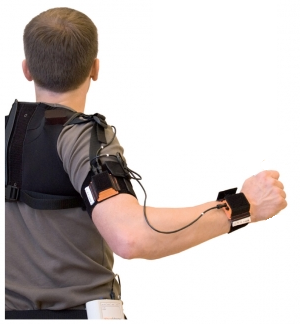
\includegraphics[scale=0.4]{../img/xsens_brazo.png} 
			\end{center}
		\end{column}
		\begin{column}{3cm}
			\begin{center}
			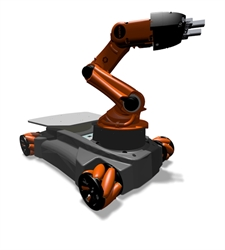
\includegraphics[scale=0.5]{../img/youbot_pres.jpeg} 
			\end{center}
		\end{column}
	\end{columns}
	\end{center}
}

\section{Cómo obtener la posición de un brazo humano}
\subsection{Cómo obtener la posición de un brazo humano}
\frame{\frametitle{\textbf{Cómo obtener la posición de un brazo humano}}
	\begin{columns}
		\begin{column}{3cm}
			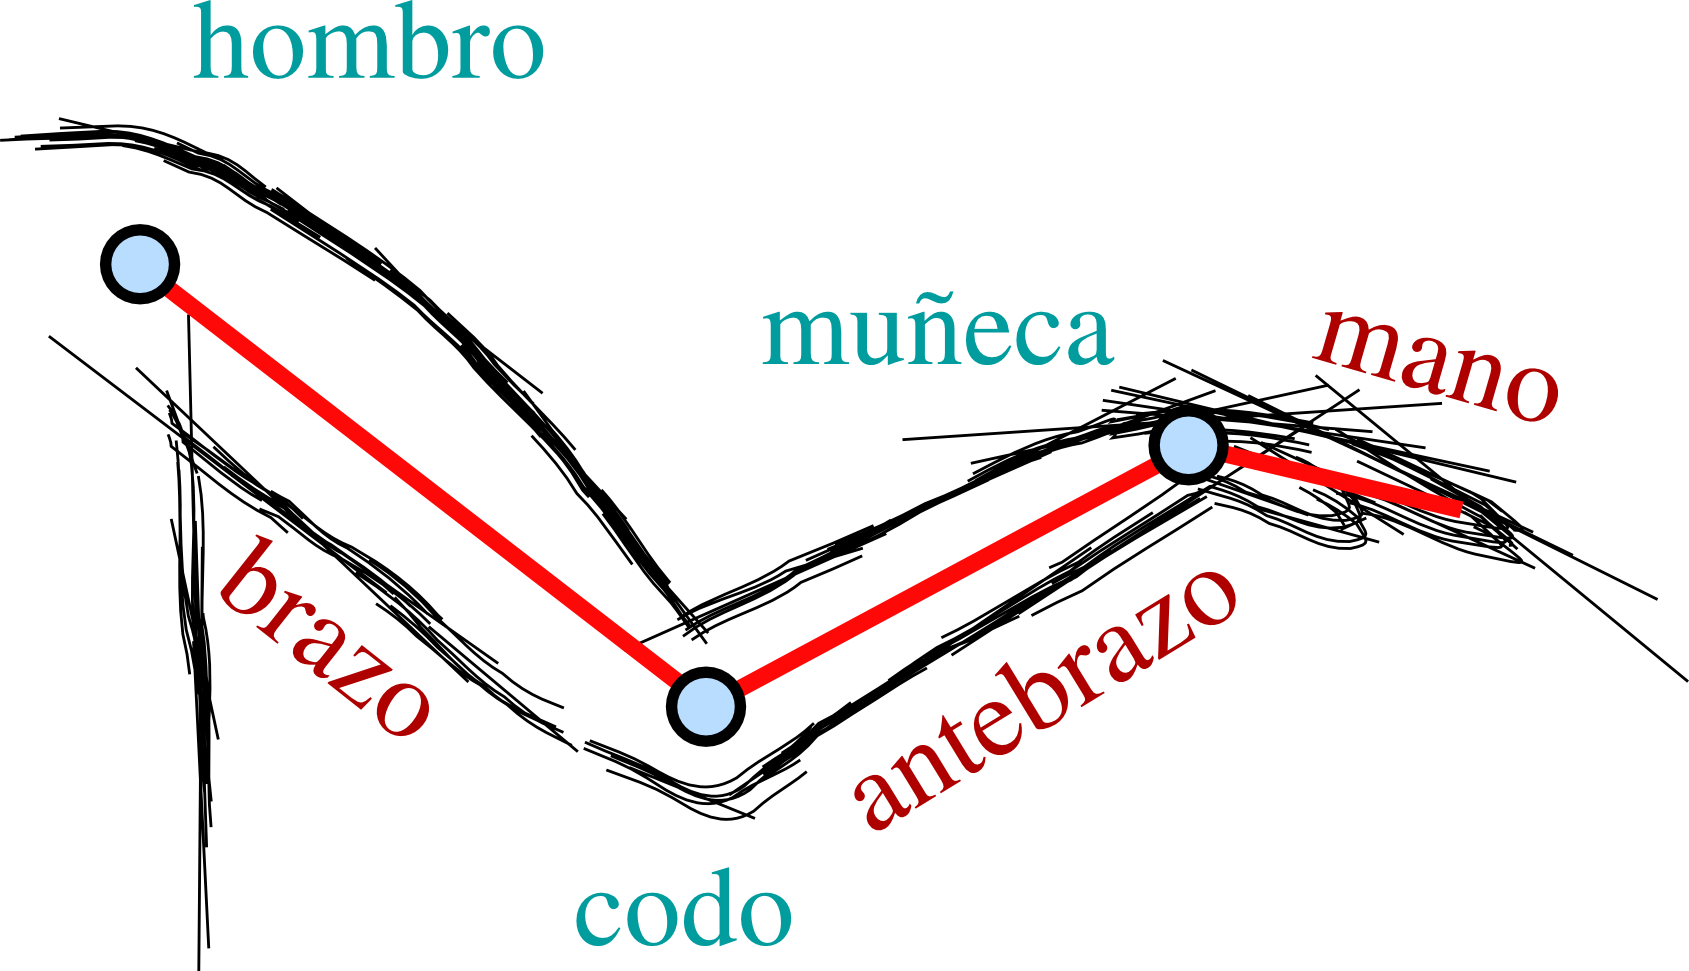
\includegraphics[scale=0.25]{../img/brazo.png} 
		\end{column}
		\begin{column}{7cm}
			\begin{itemize}
				\item El brazo humano está compuesto por \textbf{3 articulaciones} (hombro, codo y muñeca) y \textbf{3 eslabones} (brazo, antebrazo y mano).
				\item Se puede definir la posición del brazo mediante las \textbf{orientaciones} de sus tres eslabones.
				
				\item No se tendrán en cuenta las \textbf{longitudes}, ya que estas \textbf{no varían con el tiempo}.
			\end{itemize}
		\end{column}
	\end{columns}
}

\subsection{Qué se entiende por orientación}
\frame{\frametitle{\textbf{Qué se entiende por orientación}}
	\begin{columns}
		\begin{column}{3cm}
			
			
			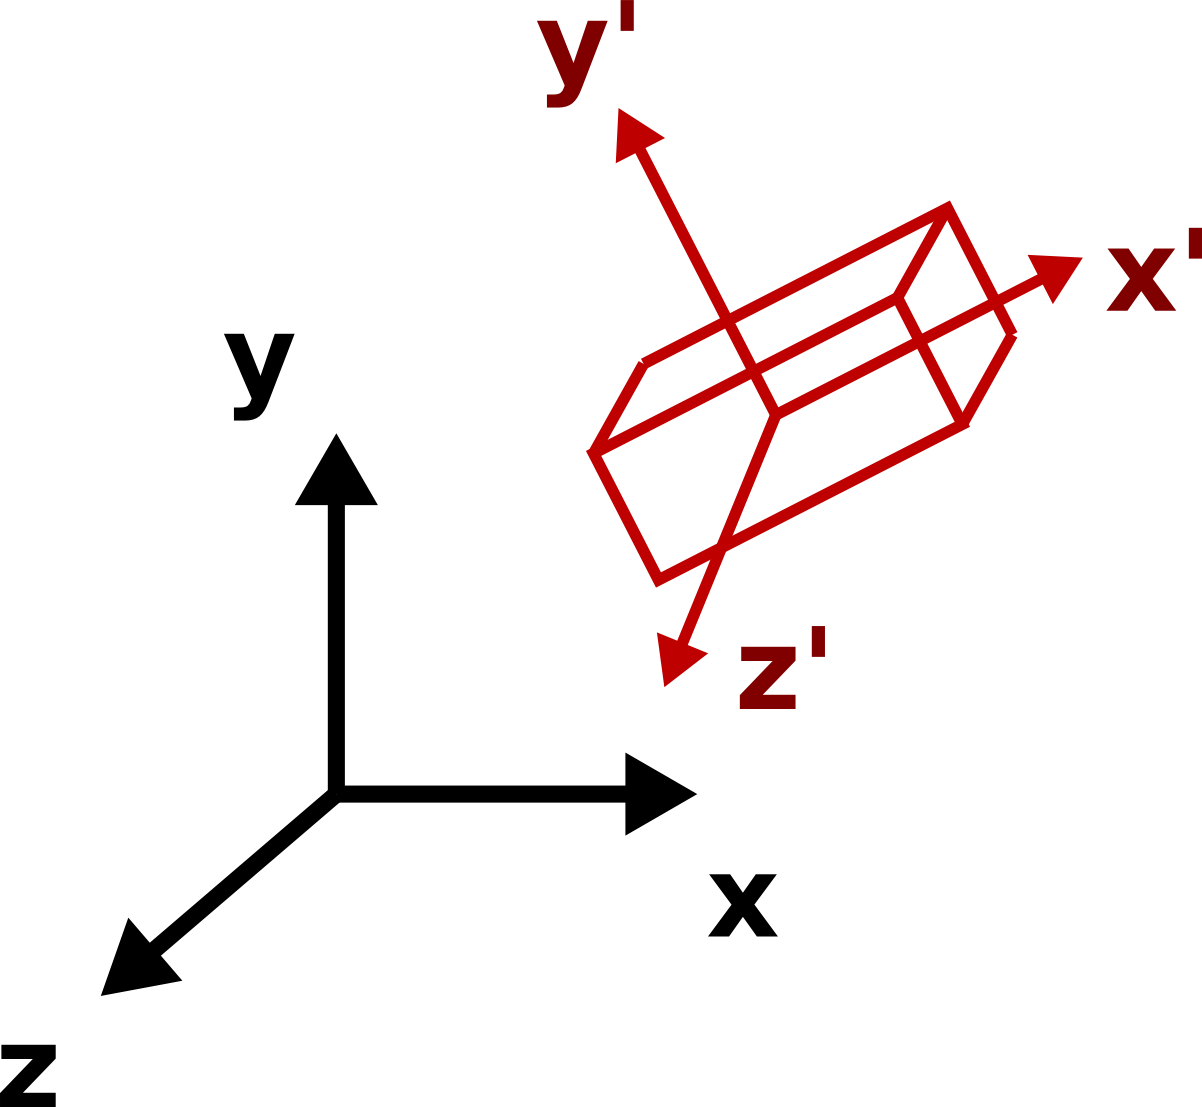
\includegraphics[scale=0.5]{../img/orientacion.png}\\
			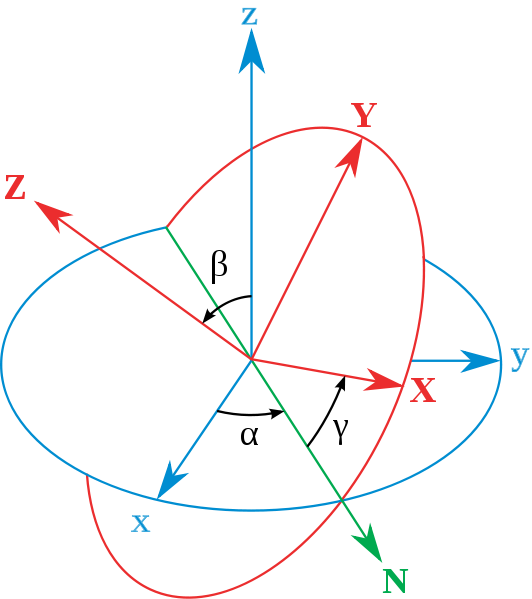
\includegraphics[scale=0.15]{../img/angulos_euler.png} 
		\end{column}
		\begin{column}{7cm}
			\begin{itemize}
				\item La \textbf{orientación} de un cuerpo es una \textbf{descripción matemática} de la forma en que está situado en el espacio.
				\item Una forma de expresar la orientación es mediante los ángulos que forman los ejes principales de los sistemas de referencia global y local entre sí. A estos ángulos se les llama \textbf{ángulos de Euler}. Existe el problema del \textbf{gimbal lock}.
				\item Existen otras formas de representación de la orientación más robustas que no presentan el inconveniente del \textbf{gimbal lock}, como las matrices de rotación o los cuaterniones. En este proyecto se escogerán los \textbf{cuaterniones}.
			\end{itemize}
		\end{column}
	\end{columns}
}

\subsection{Cómo obtener otras magnitudes con los cuaterniones de orientación}
\frame{\frametitle{\textbf{Cómo obtener otras magnitudes con los cuaterniones de orientación}}
	\begin{columns}[T]
		\begin{column}{4cm}
			
			%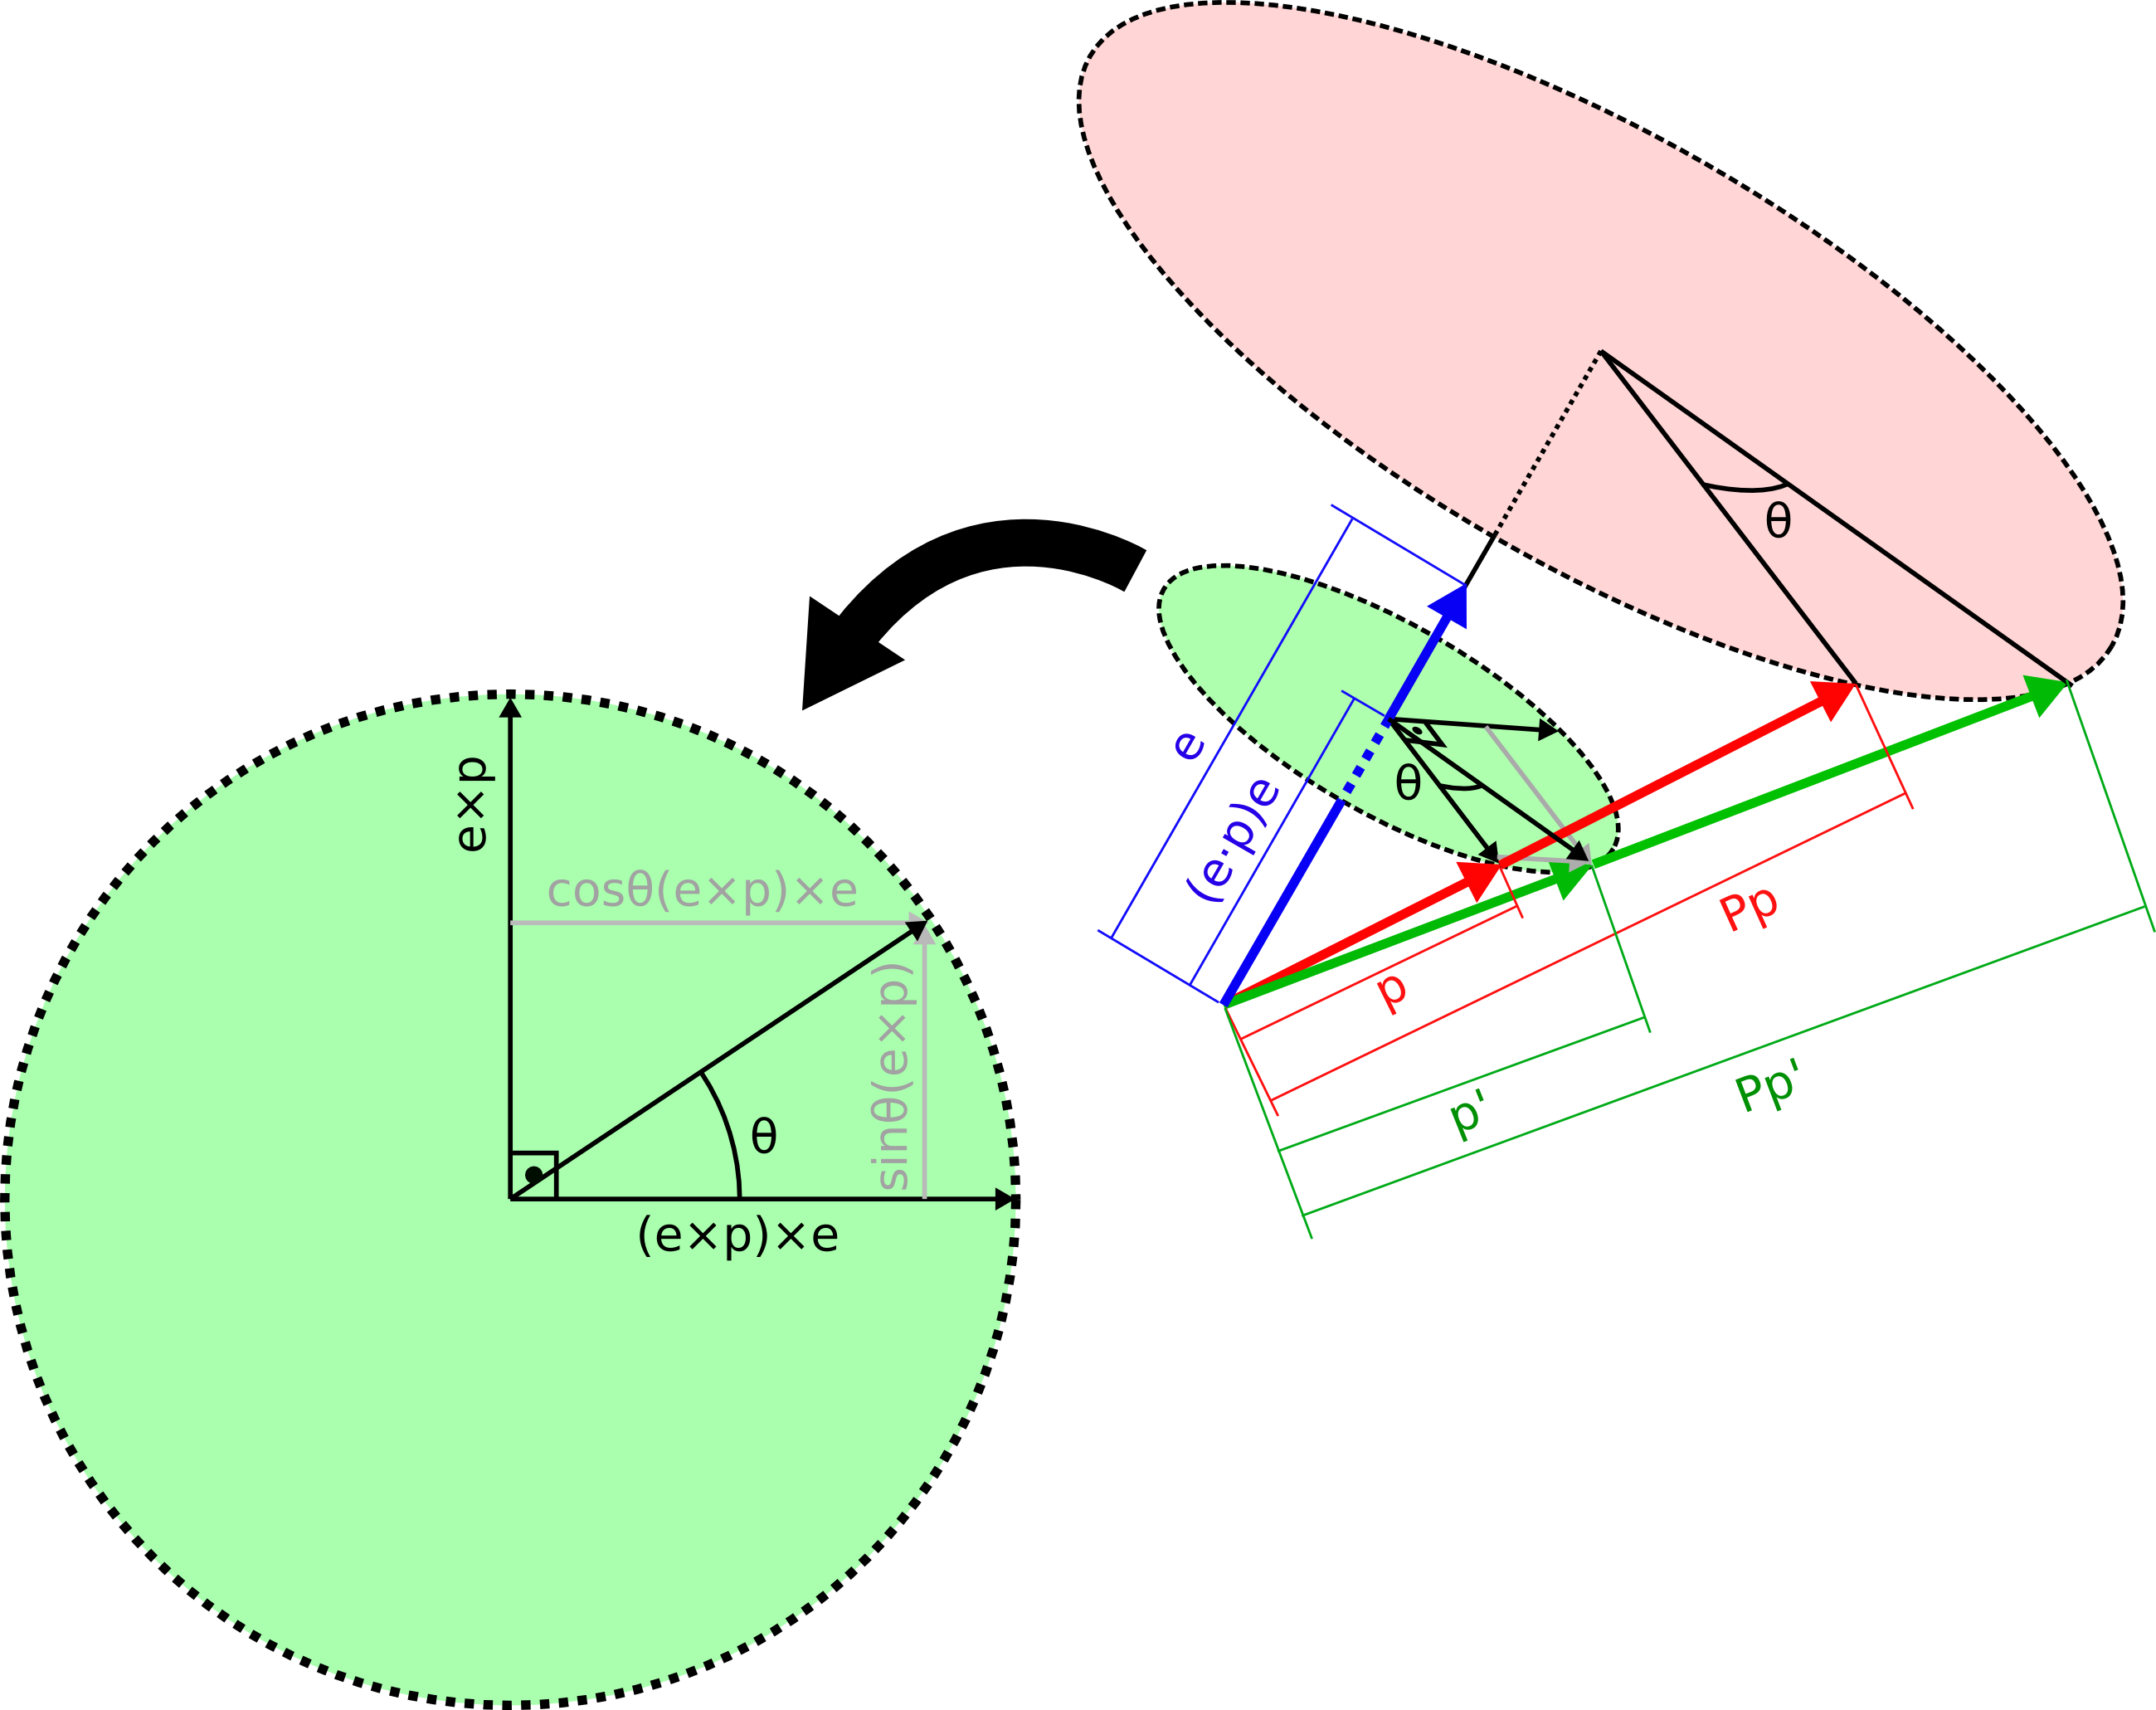
\includegraphics[scale=0.4]{../img/rotation_quaternion.png} \\
			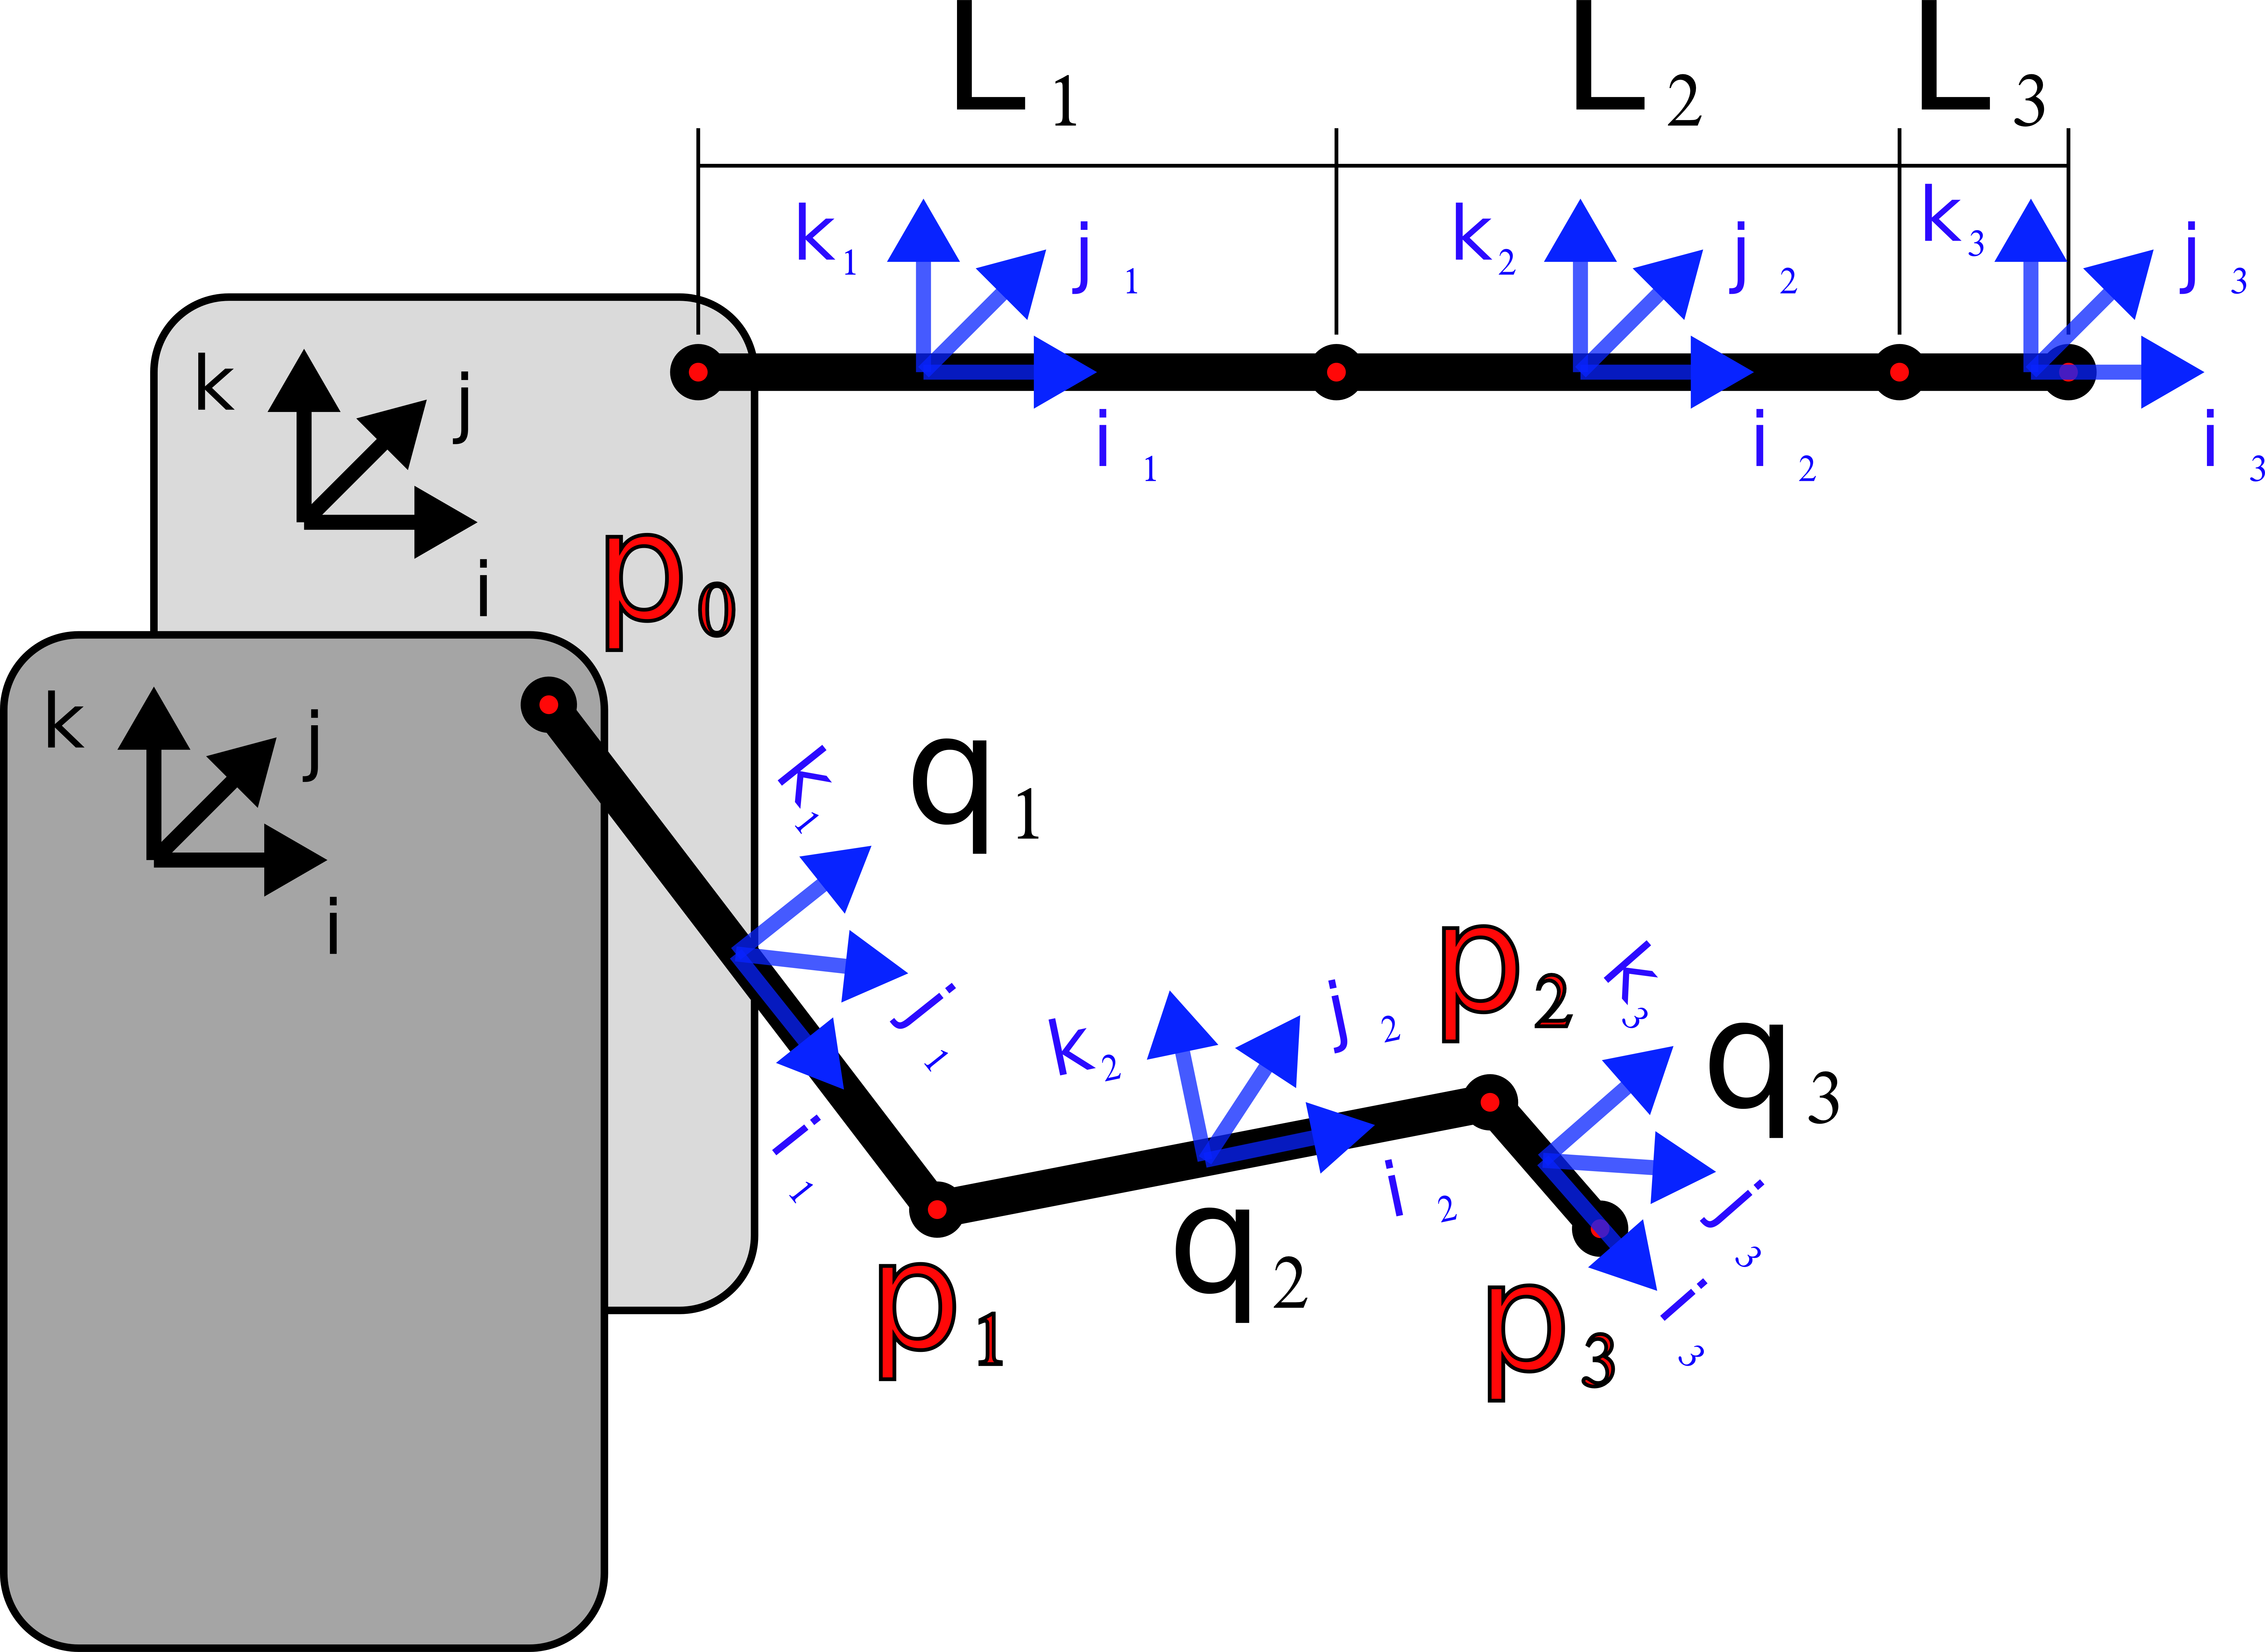
\includegraphics[scale=0.25]{../img/arm_position.png}
			
			
		\end{column}
		\begin{column}{6cm}
			\footnotesize
			Con los cuaterniones de orientación es fácil obtener otras magnitudes del brazo.
			\begin{itemize}
				\item Posición de cualquier punto del brazo: $p_G = q_kp_L^iq_k^* + \sum\limits_{m = 1}^{k-1} q_m (L_mi) q_m^* $
				\item Velocidad lineal de un punto del brazo: $v(p) = \frac{1}{\Delta t}\left( p_k - p_{k-1}\right)$
				\item Velocidad angular de un eslabón: $ \xi = q_{k-1}^*q_k = c_{\xi} + s_{\xi}e_{\xi} \iff $ $\omega = \frac{2}{\Delta t} \arctan \left( \frac{s_{\xi}}{c_{\xi}} \right) e_{\xi}$
			\end{itemize}
			\normalsize
		\end{column}
	\end{columns}
}

\subsection{Cómo obtener los ángulos de Euler a partir de los cuaterniones de orientación}
\frame{\frametitle{\textbf{Cómo obtener los ángulos de Euler a partir de los cuaterniones de orientación}}
	\scriptsize	
	\begin{columns}
		\begin{column}{3cm}
			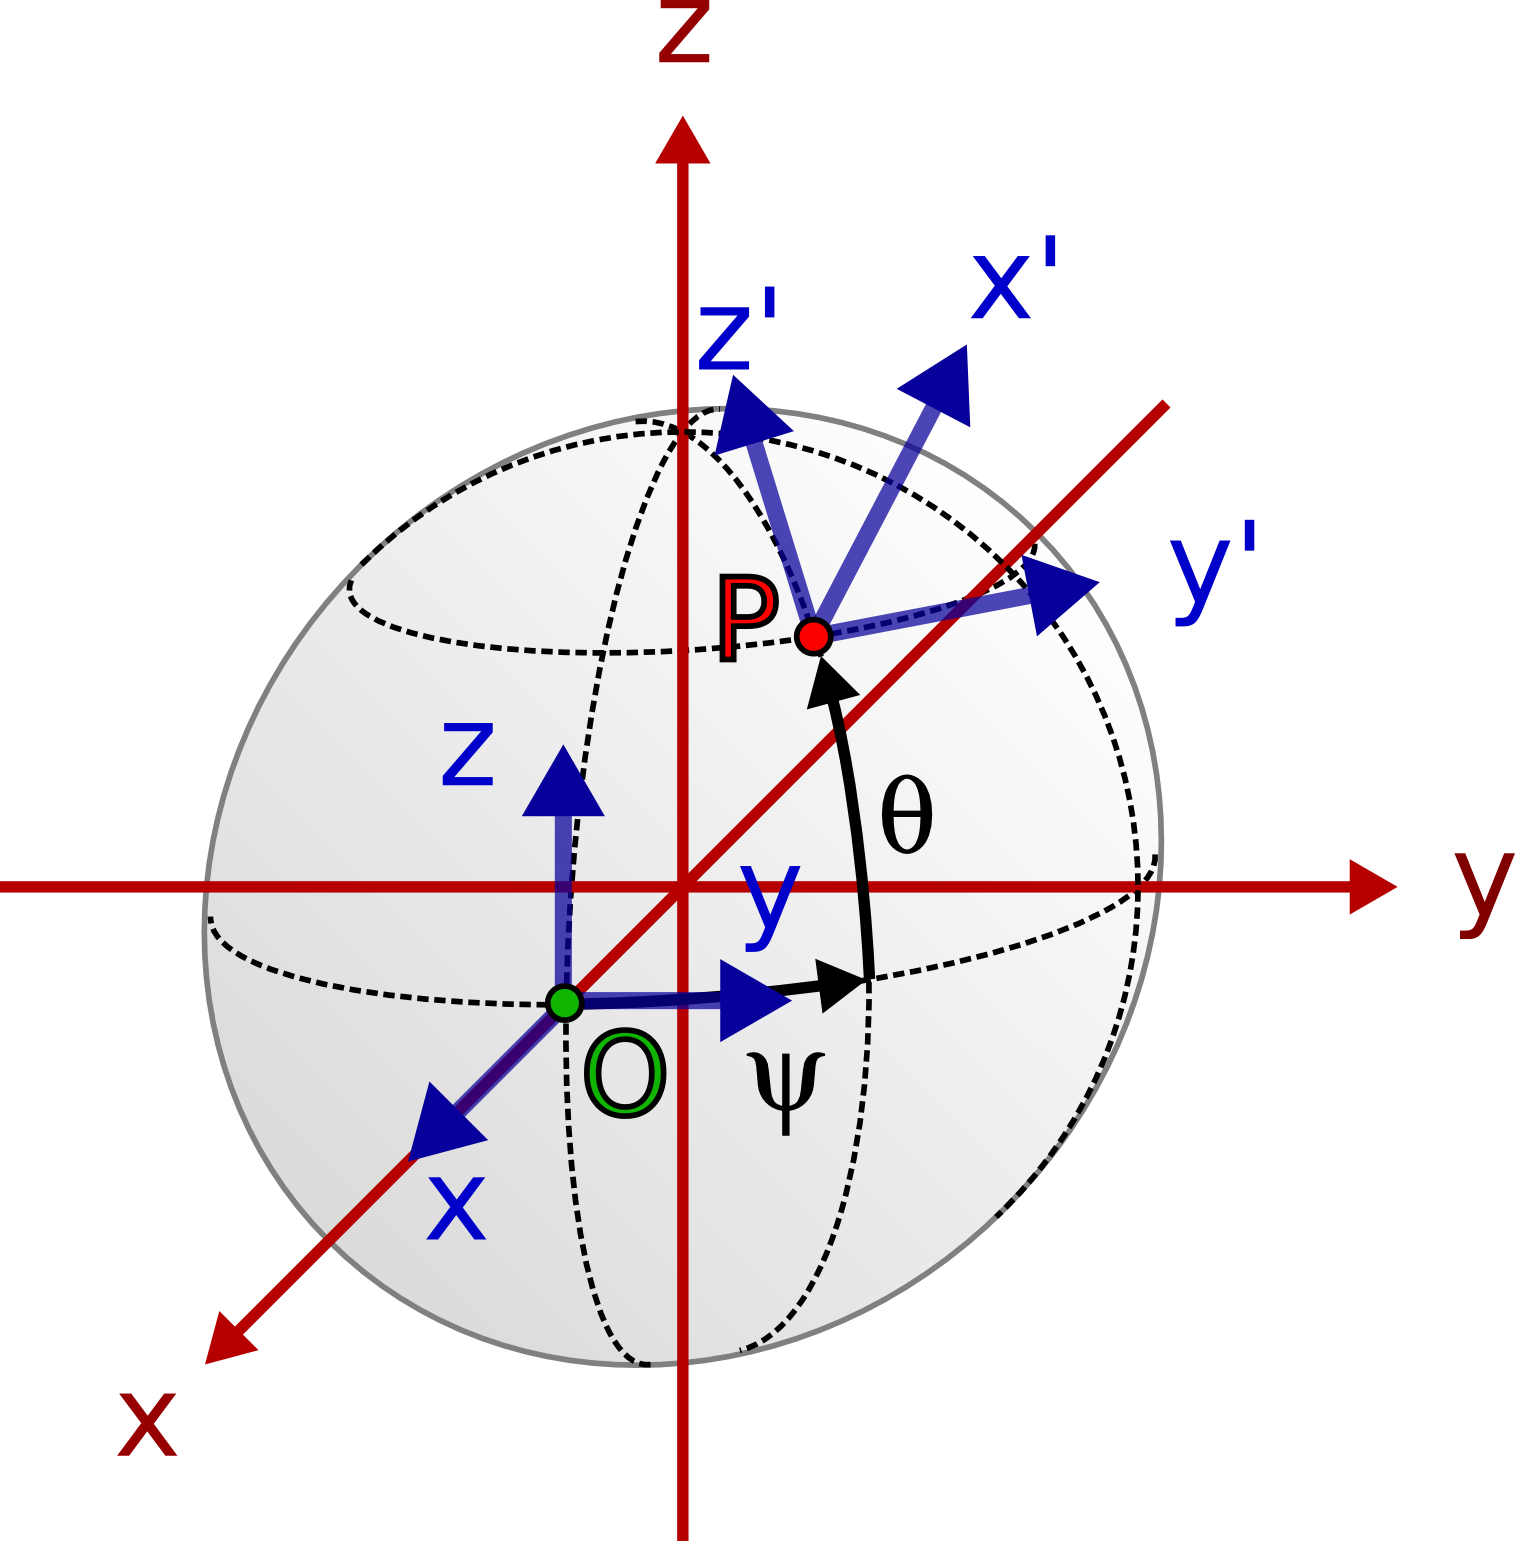
\includegraphics[scale=0.4]{../img/sphere.png} \\
		\end{column}
		\begin{column}{7cm}
			\begin{itemize}
				\item Los ángulos de Euler se utilizarán el la determinación de los ángulos que ha de tener cada articulación del robot para que cierto eslabón adopte la misma orientación que la leída por el sensor.
				\item Para la obtención de los ángulos de Euler se imaginará el sistema de coordenadas 2 situado sobre una esfera unitaria de forma que en todo momento el eje X sea normal a la esfera.
				\item Aplicando geometría se obtienen los ángulos buscados.
			\end{itemize}
		\end{column}
	\end{columns}			
			
			
			\begin{table}[h]
			\center
			\begin{tabular}{|l|l|c|}
			\hline
			\multicolumn{3}{|c|}{\textbf{Cálculo de los ángulos de Euler a partir del cuaternión de orientación}}\\
			\hline
			1º & Cálculo de $i''$ y $j''$ & $ i' = i'' = q_siq_s^* \quad j'' = q_sjq_s^*$  \\
			2º & Obtención de los ángulos $\psi$ y $\theta$ & $ \psi = \arctan \left( \displaystyle\frac{i'_y}{i'_x} \right) \quad \theta = \arcsin i'_z $ \\
			3º & Cálculo del vector $j'$ y $k'$ & $ j' = \displaystyle\frac{1}{\cos\theta} \left( - i''_y i + i''_x j \right) \quad k' = i' \times j' $ \\
			4º & Obtención del tercer ángulo, $\phi$ & $ \phi = \arctan \displaystyle\frac{j'' \cdot k'}{j'' \cdot j'} $ \\
			\hline
			\end{tabular}
			
			\label{tab:algoritmo_angulos_euler}
		
			\end{table}
		\normalsize

}

\subsection{¿Por qué usar cuaterniones entonces?}
\frame{\frametitle{\textbf{¿Por qué usar cuaterniones entonces?}}
	\footnotesize	
	\begin{columns}
		\begin{column}{3cm}
			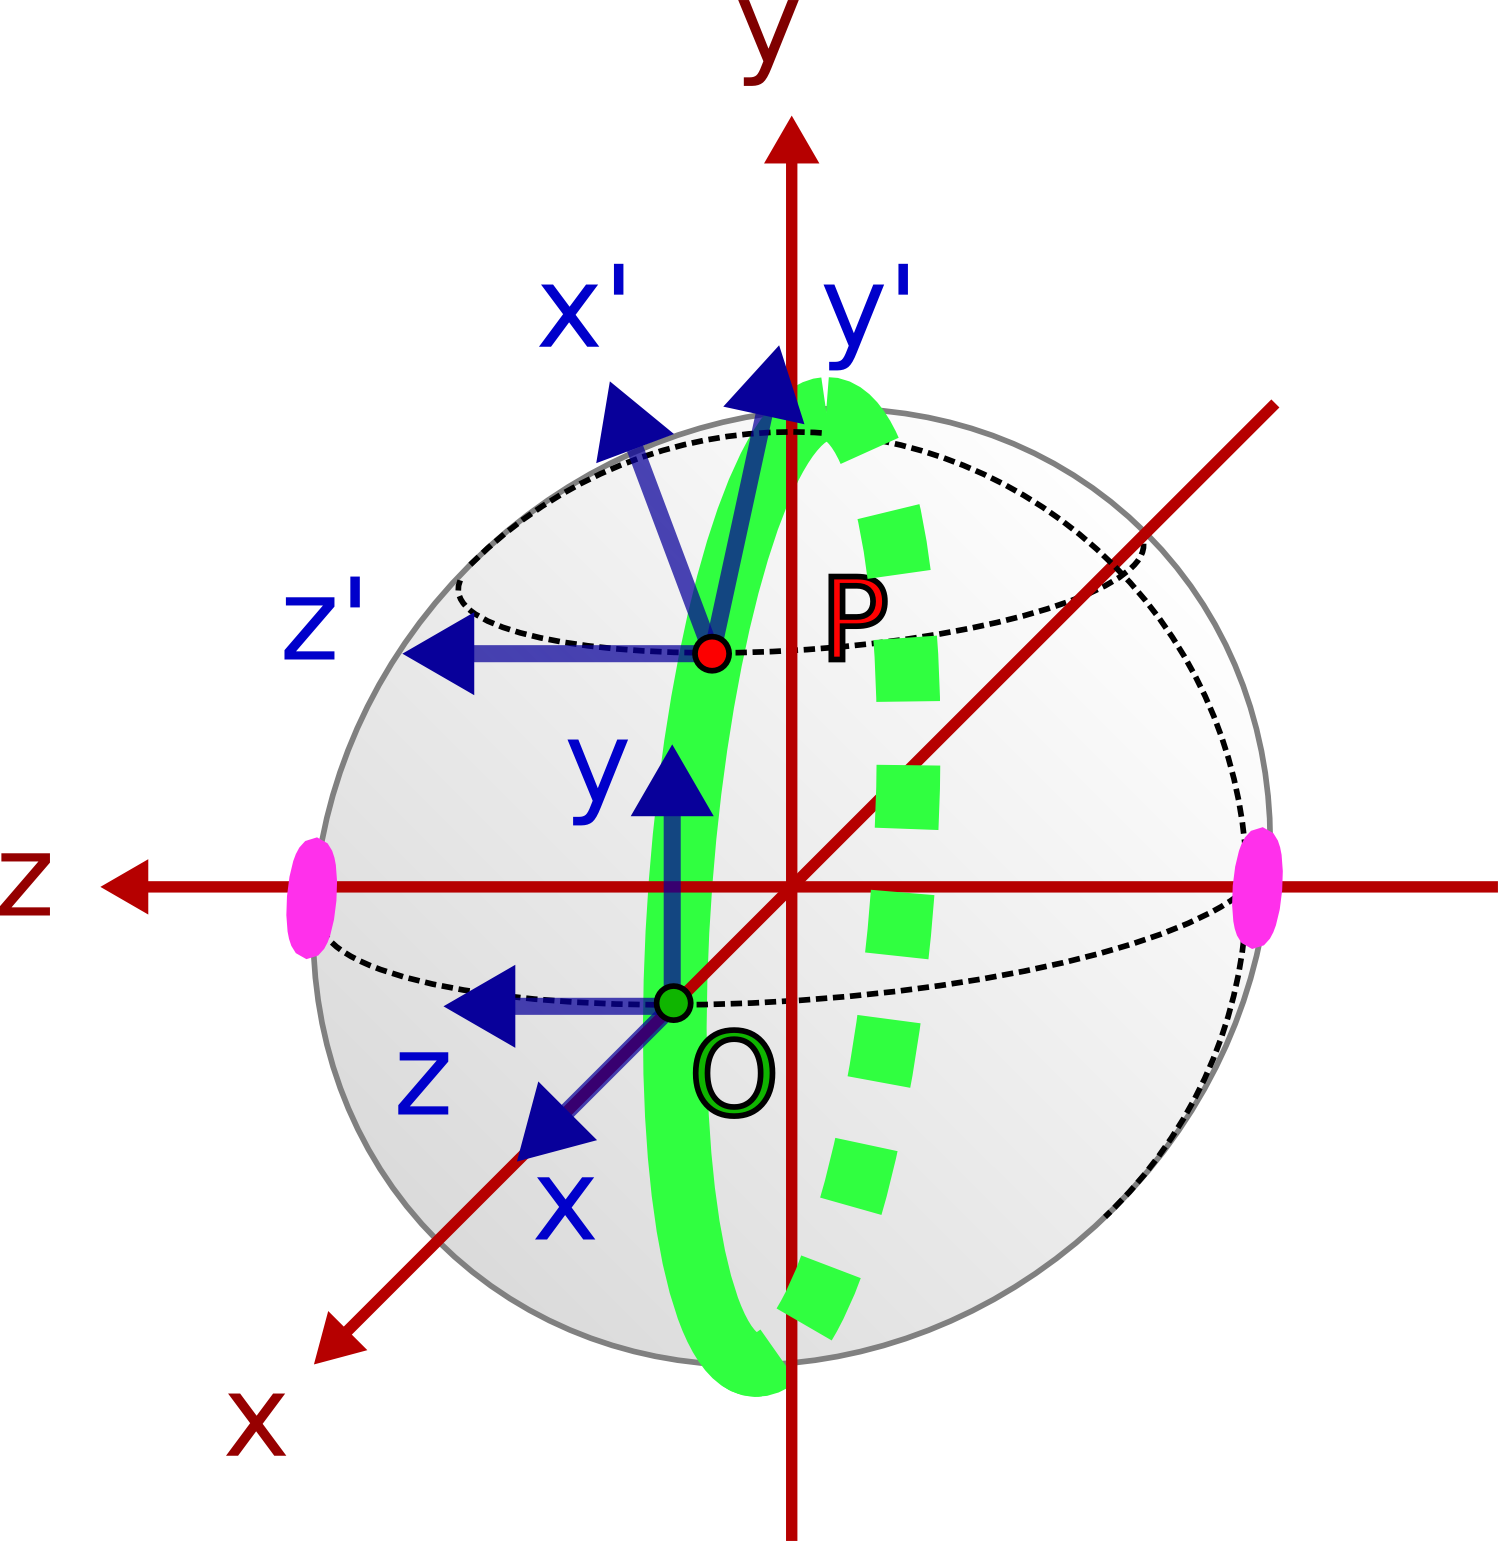
\includegraphics[scale=0.5]{../img/yaxis.png} 
		\end{column}
		\begin{column}{7cm}
			\begin{itemize}
				\item Con el algoritmo presentado anteriormente, la zona de gimbal lock se produce en los cortes del eje Z con la esfera unitaria.
				
				\item En articulaciones de un grado de libertad es posible desplazar la zona de \textit{gimbal lock} de forma que nunca se pase por ella.
				
				\item Ejemplo: articulación de rotación sobre el eje Y. Pre-rotamos los sistemas de coordenadas 1 y 2 un ángulo de $90^\circ$ alrededor del eje X. La zona de gimbal lock se habrá desplazado de forma que nunca se pasará sobre ella. 
				\item Esta pre-rotación es muy fácil de hacer con cuaterniones, pero complicada si sólo se supieran los ángulos de Euler.
			\end{itemize}
		\end{column}
	\end{columns}
	\normalsize
	
}

\subsection{Selección de sensores}
\frame{\frametitle{\textbf{Selección de sensores}}
	\footnotesize
	Características buscadas en los sensores:\\
	\begin{itemize}
	\item Que proporcionen cuaterniones de orientación
	\item Que sean de fácil colocación en el brazo.
	\item Que no dificulten el movimiento de la persona en absoluto.
	\end{itemize}
	
	Los sensores inerciales o IMUs cumplen estas características, aunque tienen el \textbf{problema de la deriva}.\\	
	
	\textbf{Solución adoptada}: red de sensores Xsens MTx + máster Xbus
	
	\begin{center}
	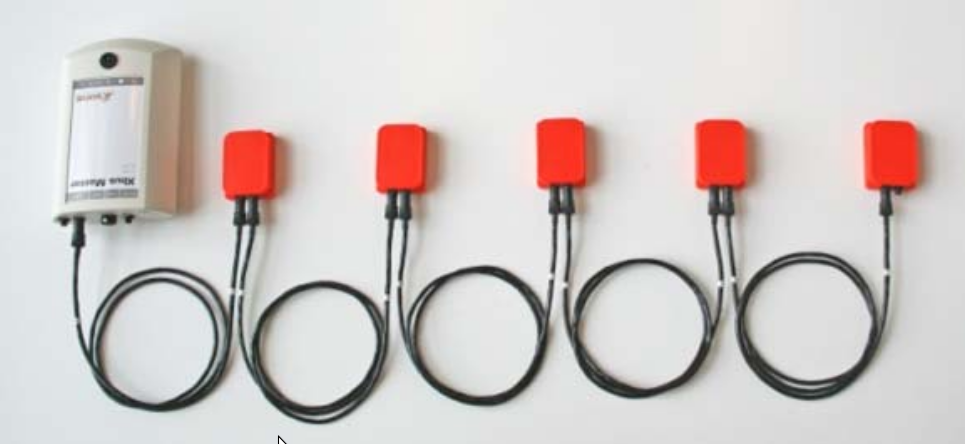
\includegraphics[scale=0.2]{../img/xbus_master.png} 
	\end{center}
	
	\begin{itemize}
	\item Eliminación de la deriva: Filtro de Kalman + corrección mediante campo magnético y aceleración gravitatoria.
	\item Error $ < 2^\circ$ en situaciones dinámicas y de $< 1^\circ$ en situaciones estáticas, según el fabricante.
	\end{itemize}
	\normalsize
}

\section{Qué es ROS y qué papel juega en el sistema de monitorización}

\subsection{Qué es la plataforma ROS}

\frame{\frametitle{\textbf{La plataforma ROS}}
	\footnotesize
	\begin{center}
	
\includegraphics[scale=1.0]{../img/Logo-ROS.png} 
	
\includegraphics[scale=0.5]{../img/willow_garage.jpeg}
	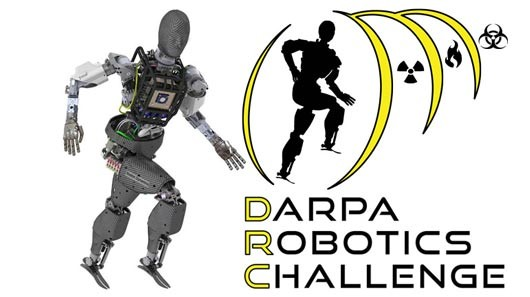
\includegraphics[scale=0.17]{../img/darpa.jpg}
	\end{center}
	\begin{itemize}
	\item ROS (Robot Operating System) es una \textbf{plataforma de desarrollo de software para robots}, de código libre y gratuita iniciada por el laboratorio de inteligencia artificial de Stanford en 2007 y continuada por el instituto Willow Garage desde 2008.
	\item En los últimos años se ha convertido en la \textbf{plataforma líder}, sobre otras como Microsoft Robotics Studio, OROCOS o Stage.
	\item Este año, el \textbf{DARPA Robotics Challenge} convocado por el \textbf{departamento de defensa de EEUU} puso como condición el uso de ROS para la participación en el concurso.
	\end{itemize}
	\normalsize
}

\subsection{Por qué usar ROS}
\frame{\frametitle{\textbf{¿Por qué usar ROS?}}
\scriptsize
ROS proporciona una cantidad masiva de herramientas que son de gran utilidad para el presente proyecto, como por ejemplo:
\begin{itemize}
	\item Visualización de datos.
	\item Simuladores 3D: Gazebo
	\item Comunicaciones entre programas: Arquitectura P2P.
	\item Grabación de datos.
\end{itemize}

	\begin{columns}
		\begin{column}{6cm}
			\begin{itemize}			
			\item Pero en lo que de verdad destaca ROS es en la cantidad de robots y sensores disponibles que funcionan en la plataforma.\\
			
			\item Esto permitirá expandir en un futuro la aplicación del sistema de monitorización incorporando \textbf{muchos otros robots y sensores} de forma extremadamente sencilla.\\
			
			\item Por las enormes posibilidades que nos ofrece ROS, \textbf{todo el software creado en este proyecto ha sido creado y funciona en esta plataforma}.
			\end{itemize}	
		\end{column}
		\begin{column}{5cm}
			\begin{center}
				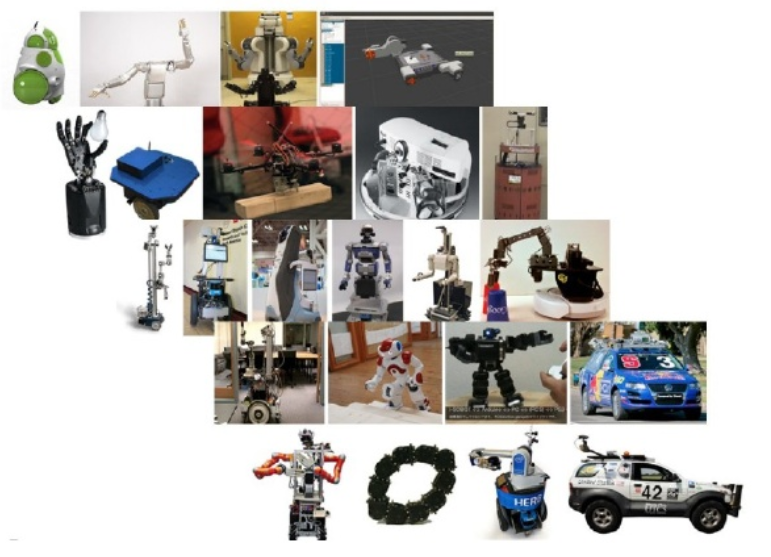
\includegraphics[scale=0.25]{../img/robots.png}
			\end{center}
		\end{column}
	\end{columns}	
	
	\normalsize
}

\subsection{¿Qué software se ha creado en ROS?}
\frame{\frametitle{\textbf{¿Qué software se ha creado en ROS?}}

	\begin{itemize}
		\item Se ha creado un driver llamado \textit{xsens\_node} para los sensores Xsens que publica en ROS los datos de los acelerómetros, giróscopos y magnetómetros, y la orientación en forma de cuaternión, matriz de orientación o ángulos de Euler (configurable).
		\item Se ha creado una librería para la obtención de datos desde otros programas de forma sencilla (librería \textit{xsens\_driver}).
		\item Además todo el aparato matemático para el manejo de vectores, matrices y cuaterniones se ha implementado en otra librería llamada \textit{dfv}.
	\end{itemize}

}

\section{Interfaz hombre-máquina utilizando el sistema de monitorización}
\frame{\frametitle{\textbf{Interfaz hombre-máquina utilizando el sistema de monitorización}}
\footnotesize
\begin{itemize}
\item La interfaz hombre-máquina que se ha creado es el resultado de combinar todos los programas y librerías desarrolladas con los sensores Xsens y el robot YouBot.

\item El robot YouBot funciona en ROS mediante un driver llamado \textit{youbot\_oodl}, con el que se puede controlar la posición de cada una de sus articulaciones desde ROS.
\end{itemize}


\begin{center}
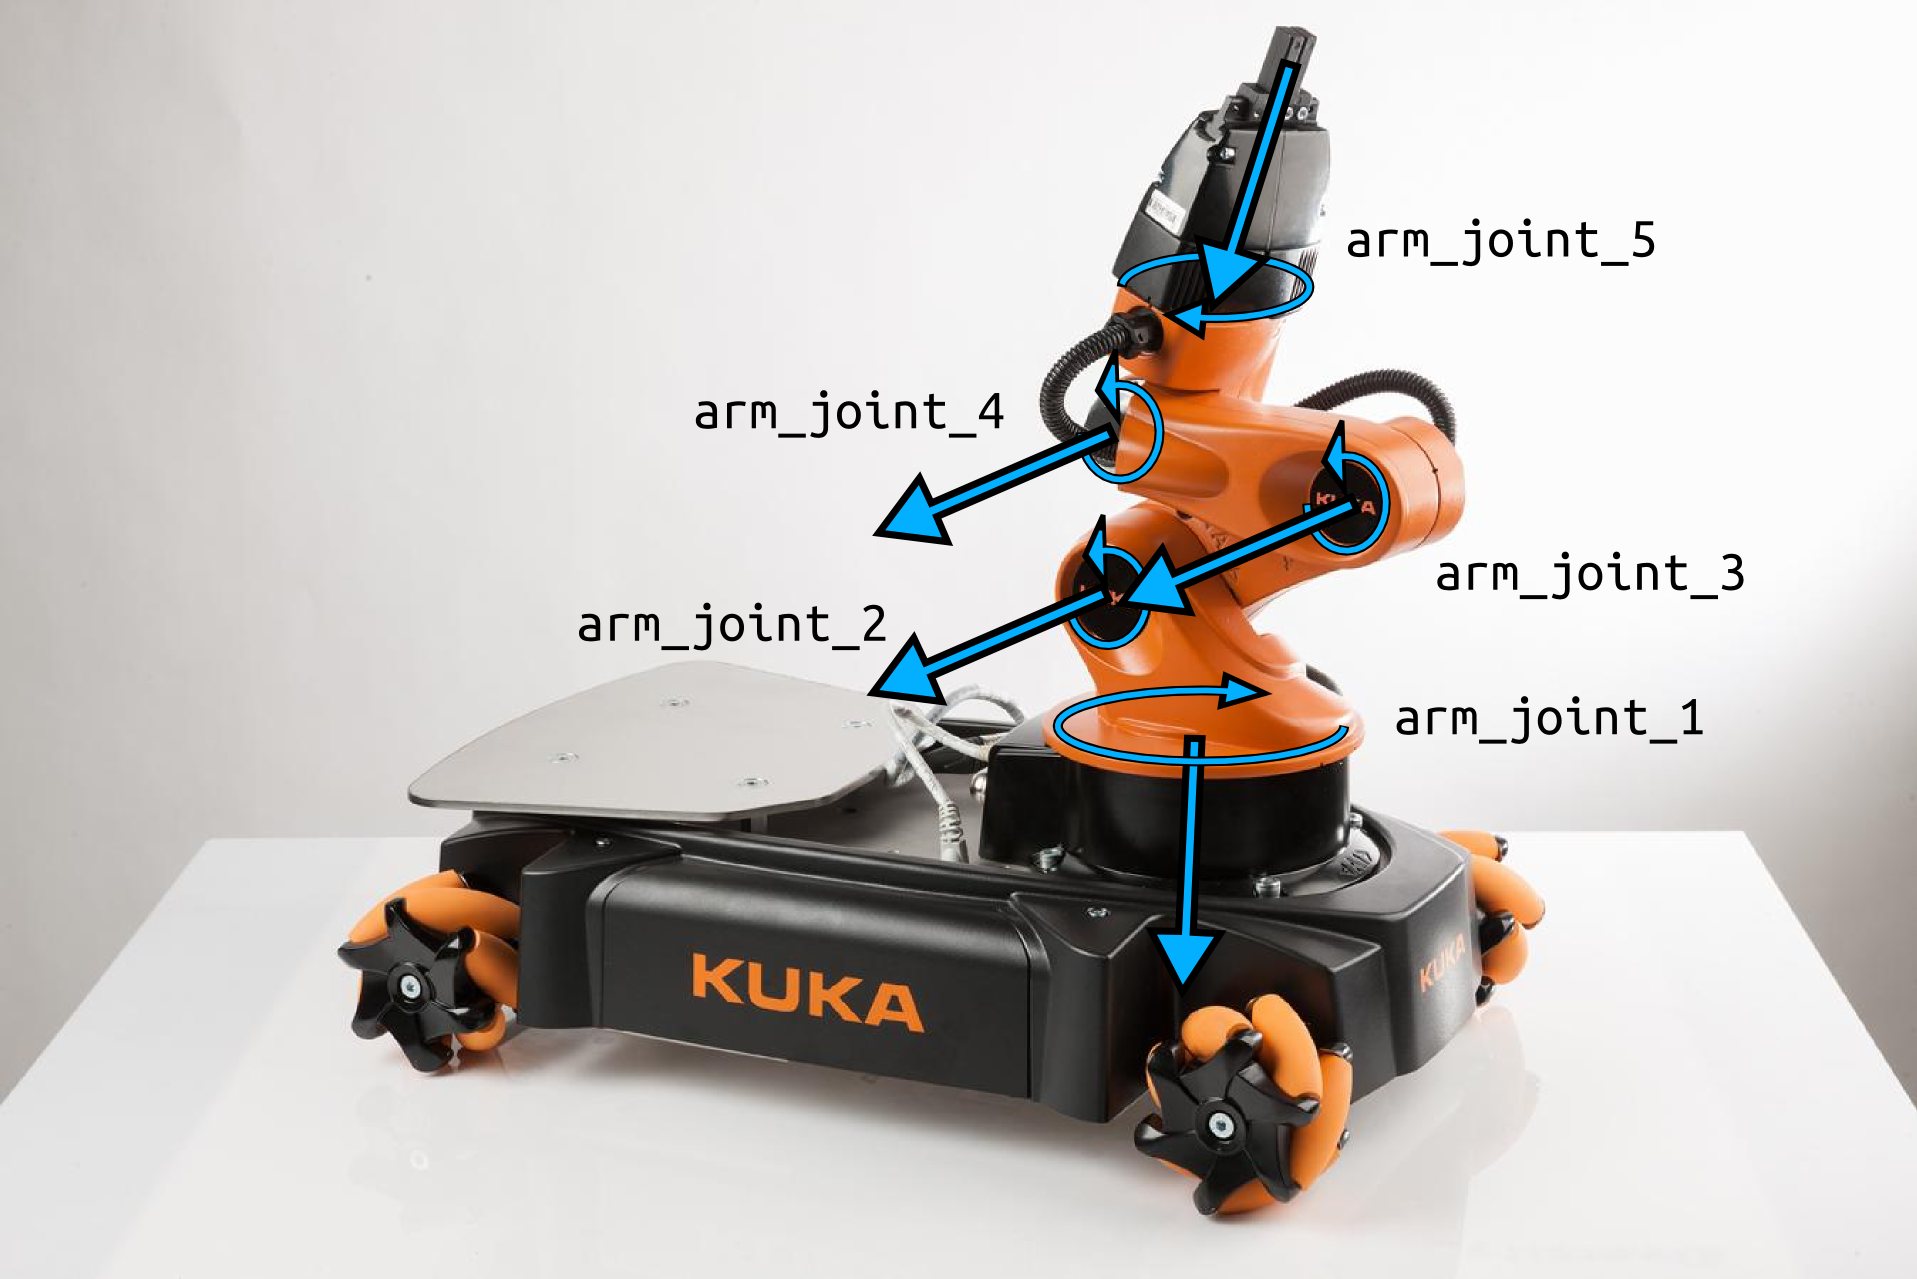
\includegraphics[scale=0.15]{../img/youbot_joints.png} 
\end{center}

\normalsize
}

\frame{\frametitle{\textbf{Interfaz hombre-máquina utilizando el sistema de monitorización}}
\footnotesize
\begin{itemize}
\item Sólo ha sido necesario crear un programa de ROS que tome por entrada los cuaterniones de orientación del driver \textit{xsens\_node}, y calcule con ellos las posiciones de cada articulación de YouBot.

\item El resultado es que mediante el movimiento del brazo se pueden controlar las articulaciones correspondientes del YouBot.
\end{itemize}

\begin{columns}
	\begin{column}{4cm}
		\begin{itemize}
			\item Se han creado otras aplicaciones extra, como un visualizador de la posición del brazo humano, y un simulador del brazo robótico del YouBot en el simulador 3D Gazebo.
			\item Gracias a ROS cada programa puede ejecutarse en un ordenador diferente.
		\end{itemize}
	\end{column}
	\begin{column}{6cm}
		\begin{center}
		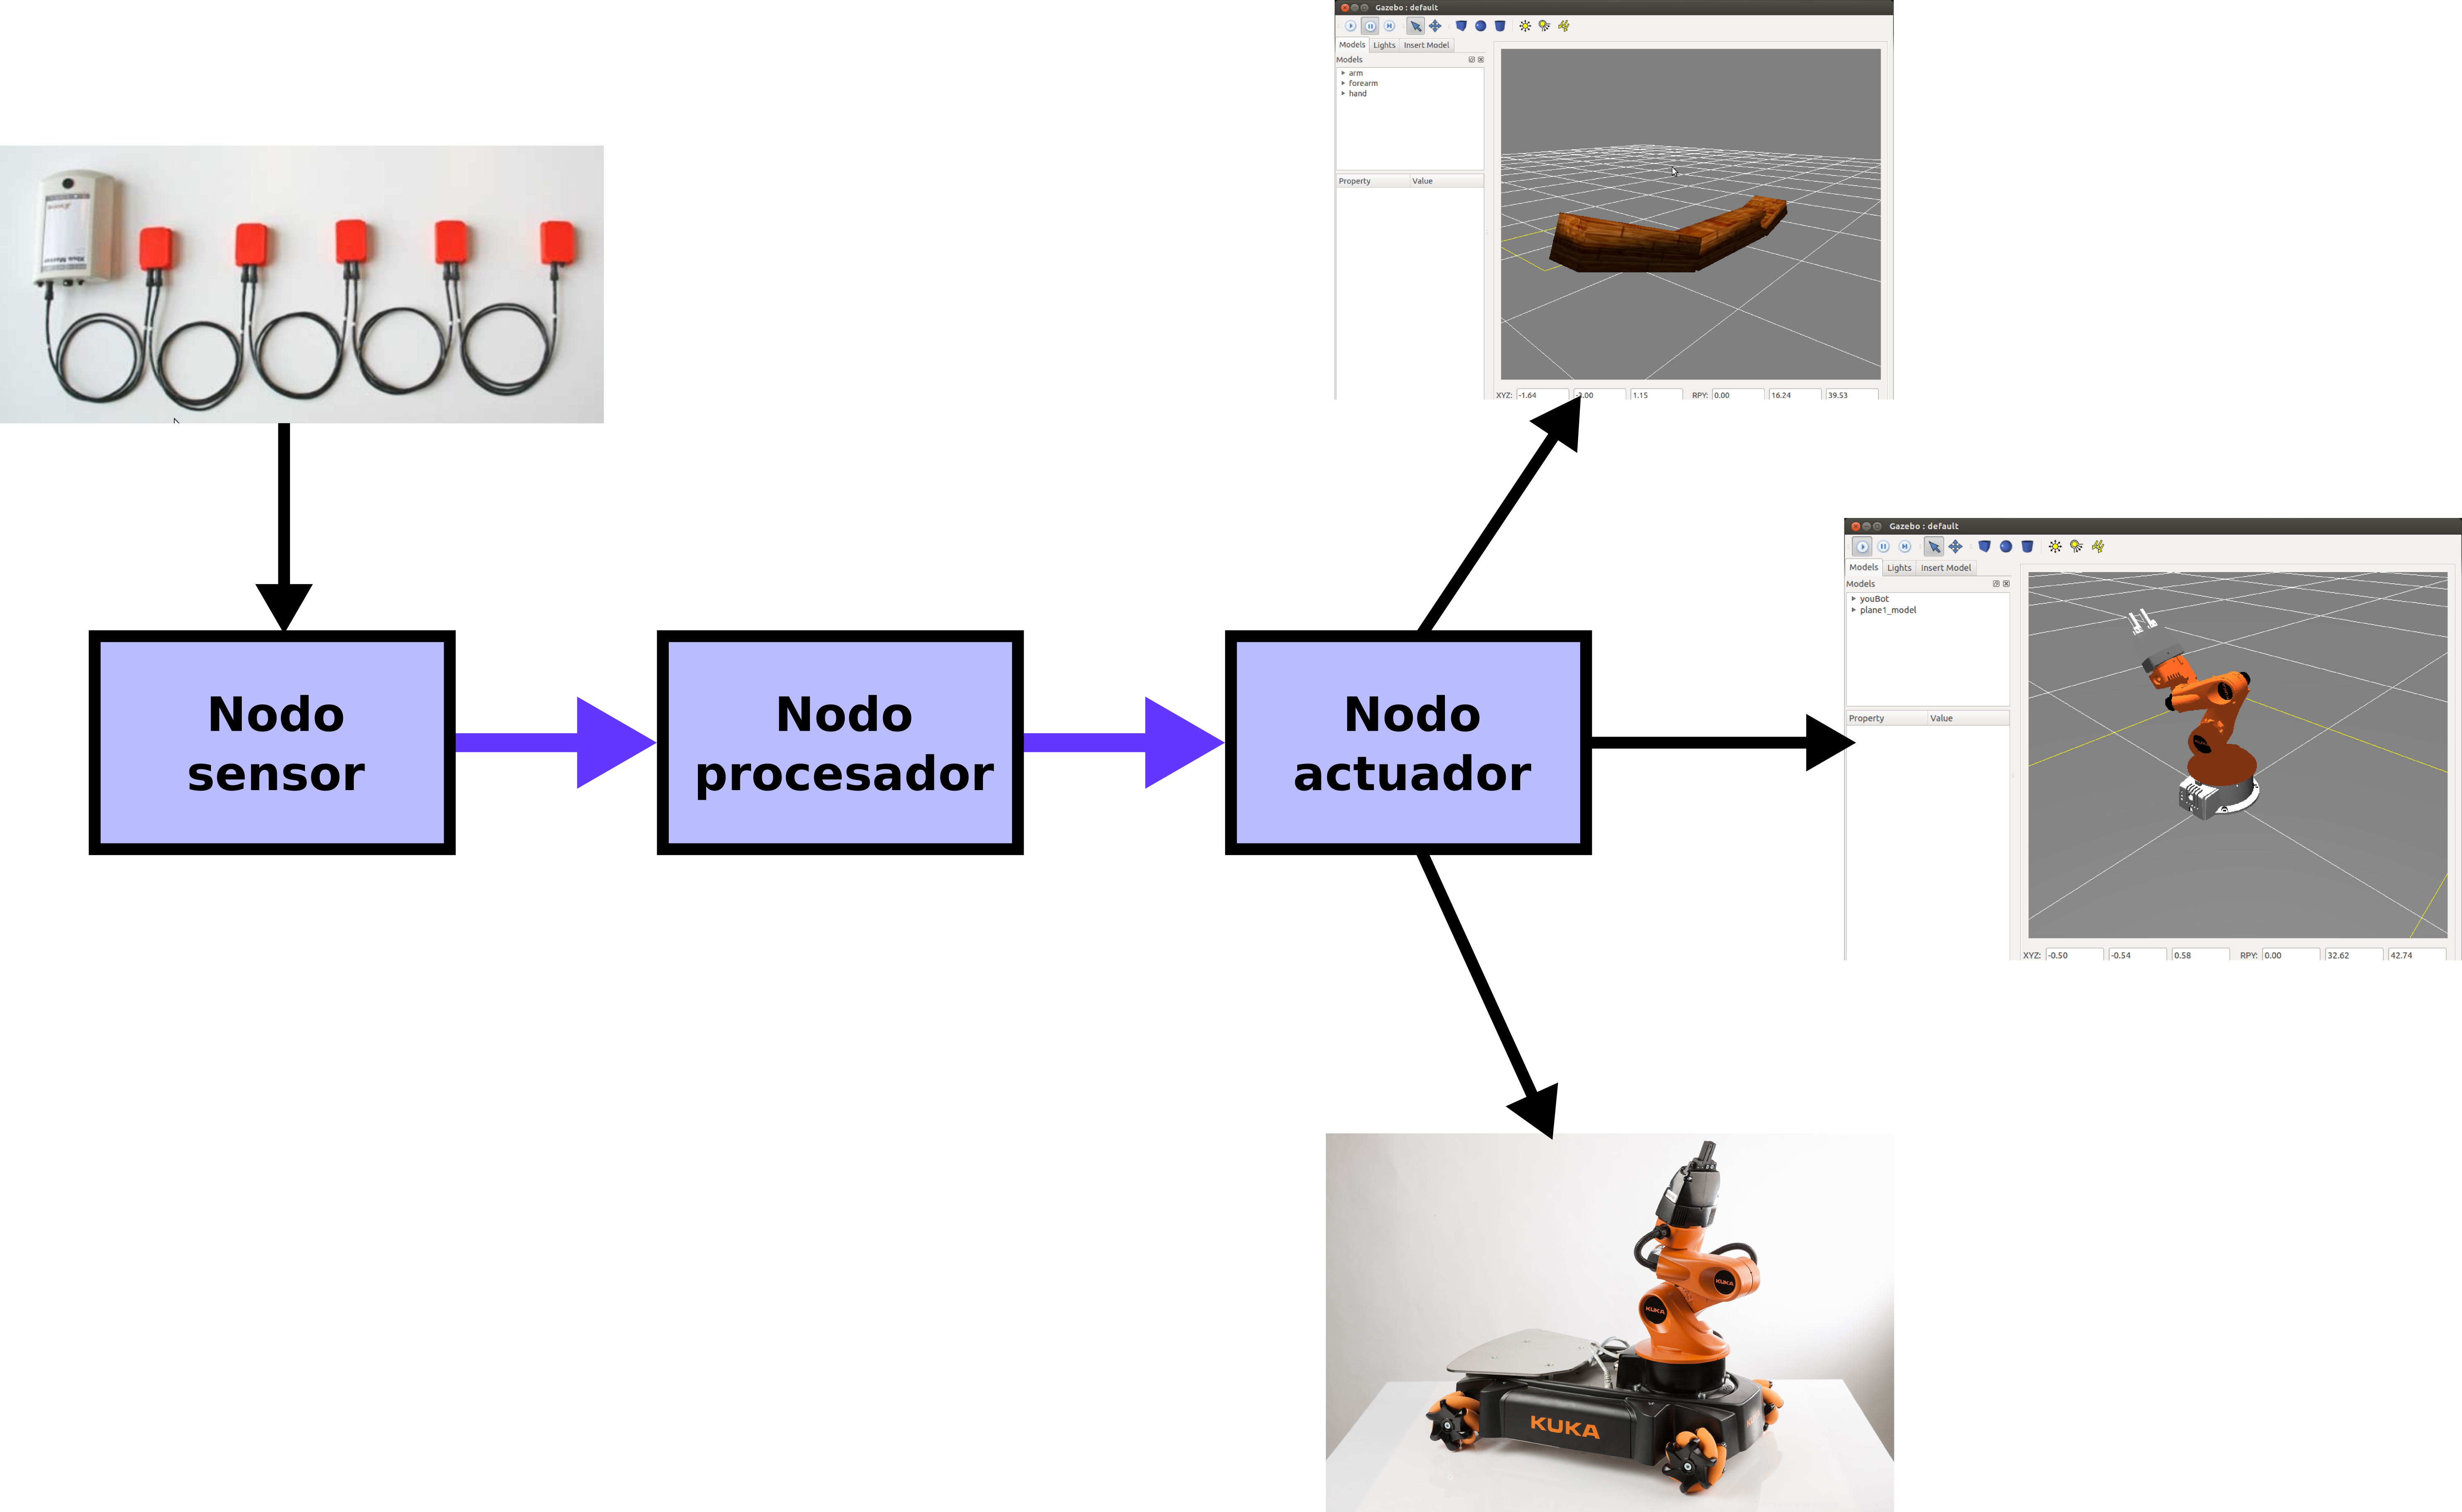
\includegraphics[scale=0.2]{../img/aplicaciones.png} 
		\end{center}
	\end{column}
\end{columns}



\normalsize
}

\section{Conclusión y trabajo futuro}
\subsection{Conclusión}
\frame{\frametitle{\textbf{Conclusión}}
	\footnotesize
	\begin{itemize}
		\item Se ha creado un sistema de monitorización \textbf{fiable} y de alta \textbf{flexibilidad} que funciona en la plataforma ROS.
		\item Se trata de un producto orientado al \textbf{desarrollador} (de ahí la creación de librerías para facilitar la toma de datos y su procesamiento, y las herramientas de visualización).
		\item Ofrece la posibilidad de incorporar \textbf{más sensores} o sensores de \textbf{distinto tipo}.
		\item Es posible incorporar el sistema en otras \textbf{aplicaciones} de forma sencilla.
		\item Su arquitectura que posibilita la creación de un \textbf{sistema distribuido}.
		\item Además ha demostrado su eficacia en su aplicación en una \textbf{interfaz hombre-máquina} para teleoperación de robots.
	\end{itemize}
	\normalsize
}

\subsection{Trabajo futuro}
\frame{\frametitle{\textbf{Trabajo futuro}}
\begin{itemize}
	\item Debido a la flexibilidad del sistema, no tiene por qué restringirse a un brazo humano y sus limitaciones de movimiento. La posibilidad de incorporar más sensores da pie a utilizarlo en modelos de robots para lograr un control más preciso, consiguiendo una teleoperación del robot real controlando el movimiento del modelo.
	\item En el uso de modelos de robots, podrían incluso incorporase feedbacks de fuerza en el modelo, de modo que la percepción del entorno por parte del operador del modelo del robot sea más completa.
	\item Dada la gran cantidad de sensores y robots capaces de funcionar con ROS, las posibilidades que se abren son prácticamente infinitas.
	\end{itemize}
	
}

\frame{\frametitle{}
\begin{center}
\Huge{\textbf{FIN}}
\end{center}
}


\end{document}